\chapter{Экспериментальный раздел}
\label{cha:research}

В данном разделе будут приведены результаты работы разработанного
программного обеспечения и поставлен эксперимент по сравнению производительности
программы от сложности моделируемой сцены. Сложность оценивается количеством комбинируемых поверхностей.

\section{Результаты работы программного обеспечения}
На рисунке \ref{fig:example_run} приведено изображение - работа программы. 
\begin{figure}
  \centering
  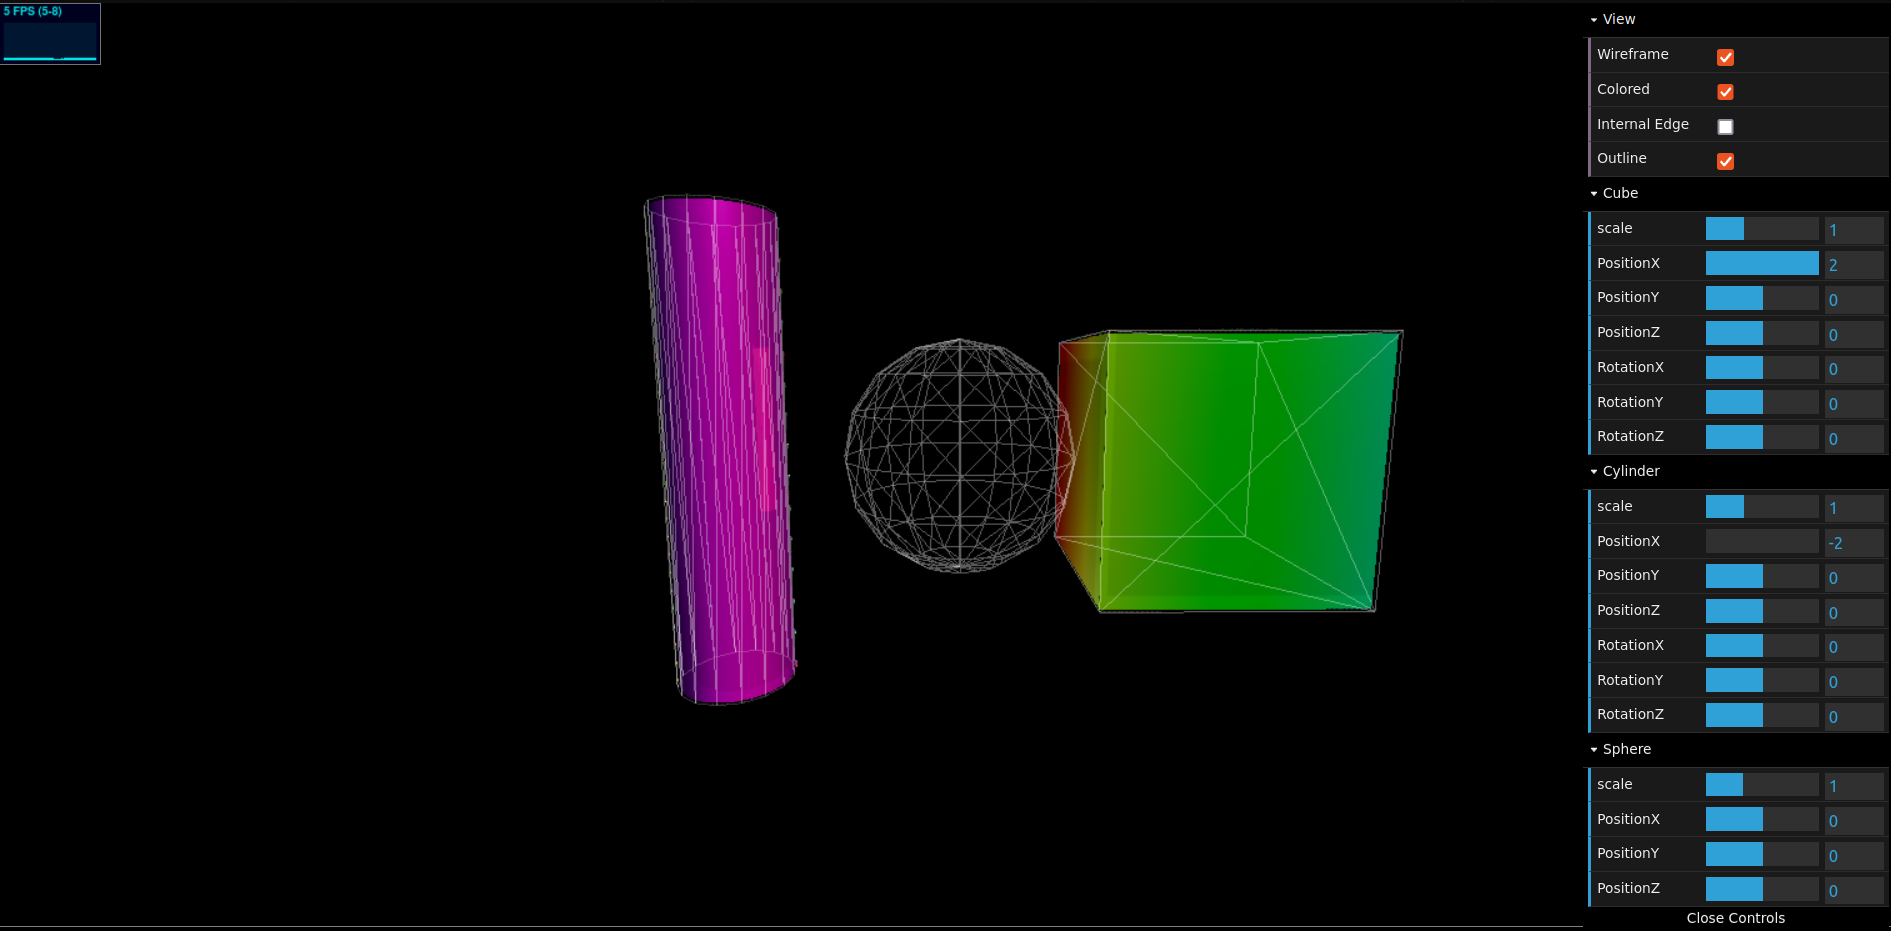
\includegraphics[scale=0.4]{inc/img/example_run}
  \caption{Демонстрация работы программы.}
  \label{fig:example_run}
\end{figure}

На сцене изображено три объекта (куб, сфера, цилиндр).
В настройках включен режим отображения каркаса, цветовая окраска.
\newpage
На рисунке \ref{fig:example_run_base} приведено изображение - композиция куба, 
сферы и цилиндра. 
На этом примере производится вычитание сферы из объединения куба и цилиндра.
\begin{figure}
  \centering
  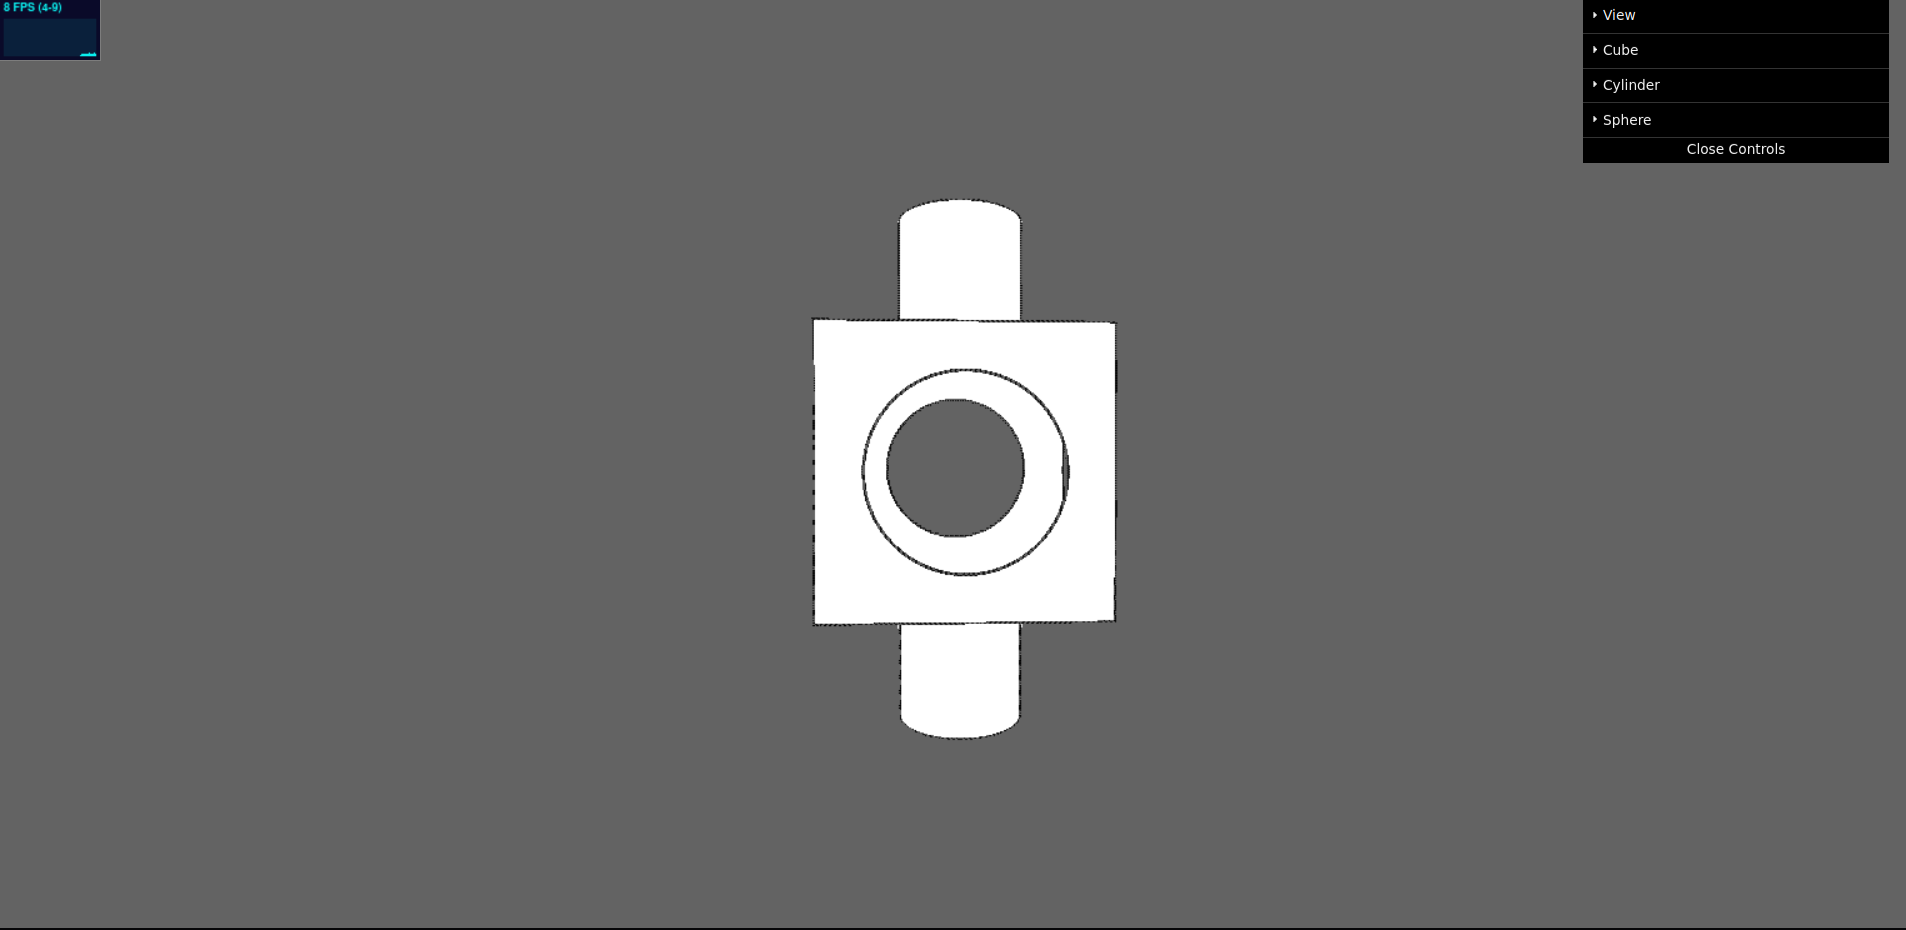
\includegraphics[scale=0.4]{inc/img/example_run_base}
  \caption{Демонстрация работы программы - композиция моделей.}
  \label{fig:example_run_base}
\end{figure}

\section{Постановка эксперимента}
\subsection{Цель эксперимента}

Целью эксперимента является проведение тестирование производительности приложения
при создании сцен разной нагруженности.  
Производительность будет оцениваться мерой количеством кадров в секунду (FPS), 
с которыми приложение работает.  
Нагрузка будет меняться в зависимости от количества объектов, расположенных на сцене.  

\subsection{Технические характеристики}

Технические характеристики устройства, на котором выполнялось тестирование:

\begin{itemize}
	\item Операционная система: Ubuntu 21.04 \cite{ubuntu} Linux \cite{linux} 64-bit.
	\item Память: 19.4 GiB.
	\item Процессор: Intel Core™ i5-8300H \cite{intel} CPU @ 2.30GHz.
	\item Видеокарты: 
  \subitem Intel(R) UHD Graphics 630 (встроенная) \cite{intel-graphics}.
  \subitem NVIDIA GeForce GTX 1050 Mobile (дискретная) \cite{nvidia-gtx1050m}.
\end{itemize}
Тестирование проводилось на ноутбуке, включенном в сеть электропитания. Во время тестирования ноутбук был нагружен только системой тестирования (работающим приложением) и системным окружением операционной системы.

\begin{table}[]
  \label{tb:comp_fps}
  \caption{Сравнение FPS при выполнении на встроенной и дискретной видеокарте.}
  \begin{tabular}{|l|l|l|l|}
  \hline
  N & Количество объектов & FPS-NVIDIA & FPS-INTEL \\
  \hline
  1 & 1                   & 60         & 15        \\
  2 & 2                   & 60         & 12        \\
  3 & 3                   & 60         & 12        \\
  4 & 4                   & 58         & 10        \\
  5 & 5                   & 52         & 8         \\
  6 & 6                   & 41         & 8         \\
  7 & 7                   & 35         & 6         \\
  8 & 8                   & 23         & 5        \\
  \hline
  \end{tabular}
\end{table}

%%% Local Variables:
%%% mode: latex
%%% TeX-master: "rpz"
%%% End:
